% Apuntes sobre el paquete beamer: http://metodos.fam.cie.uva.es/~latex/apuntes/apuntes.html (Universidad de Valladolid)
\documentclass{beamer}

\usepackage[utf8x]{inputenc}
\usepackage[T1]{fontenc}
\usepackage{lmodern}
\usepackage[spanish]{babel}
\usepackage{graphicx}

\newcommand{\software}{\textit{software }}

\mode<presentation>{\usetheme{Madrid} \setbeamercovered{dynamic}}
% Otros temas semejantes: Madrid, PaloAlto, Ilmenau

\title{\itshape Airline Common Environment}
\author{Grupo $\mathcal{D}$iedral}
\date{20 de diciembre de 2012}

\begin{document}
\maketitle

\begin{frame}
	\frametitle{Descripción general}

	\begin{block}{Resumen}
		\textit{Airline Common Environment} es un producto \software destinado a la gestión integral de una compañía aérea.	\pause
	\end{block}

	\begin{itemize}
		\item Propósito y alcance
			\begin{itemize}
				\item Gestión interna
				\item Gestión externa
			\end{itemize} \pause
		\item Perspectivas y funciones del producto \pause
		\item Características del usuario \pause
		\item Restricciones y dependencias
	\end{itemize}

	
\includegraphics[width=\paperwidth]{logoace.png}
\end{frame}

\begin{frame}
	\frametitle{Descripción general \scriptsize{ II}}

	\begin{block}{Requisitos específicos}
	\begin{itemize}
		\item Interfaces externas \pause
		\item Requisitos de rendimiento y base de datos \pause
		\item Restricciones y atributos
	\end{itemize}
	\end{block}

	
\includegraphics[width=\paperwidth]{logoace.png}
\end{frame}

\begin{frame}
	\frametitle{Gestión Interna \scriptsize{Diagrama 1}}
	
	\begin{figure}
		\hspace*{-1.2cm} 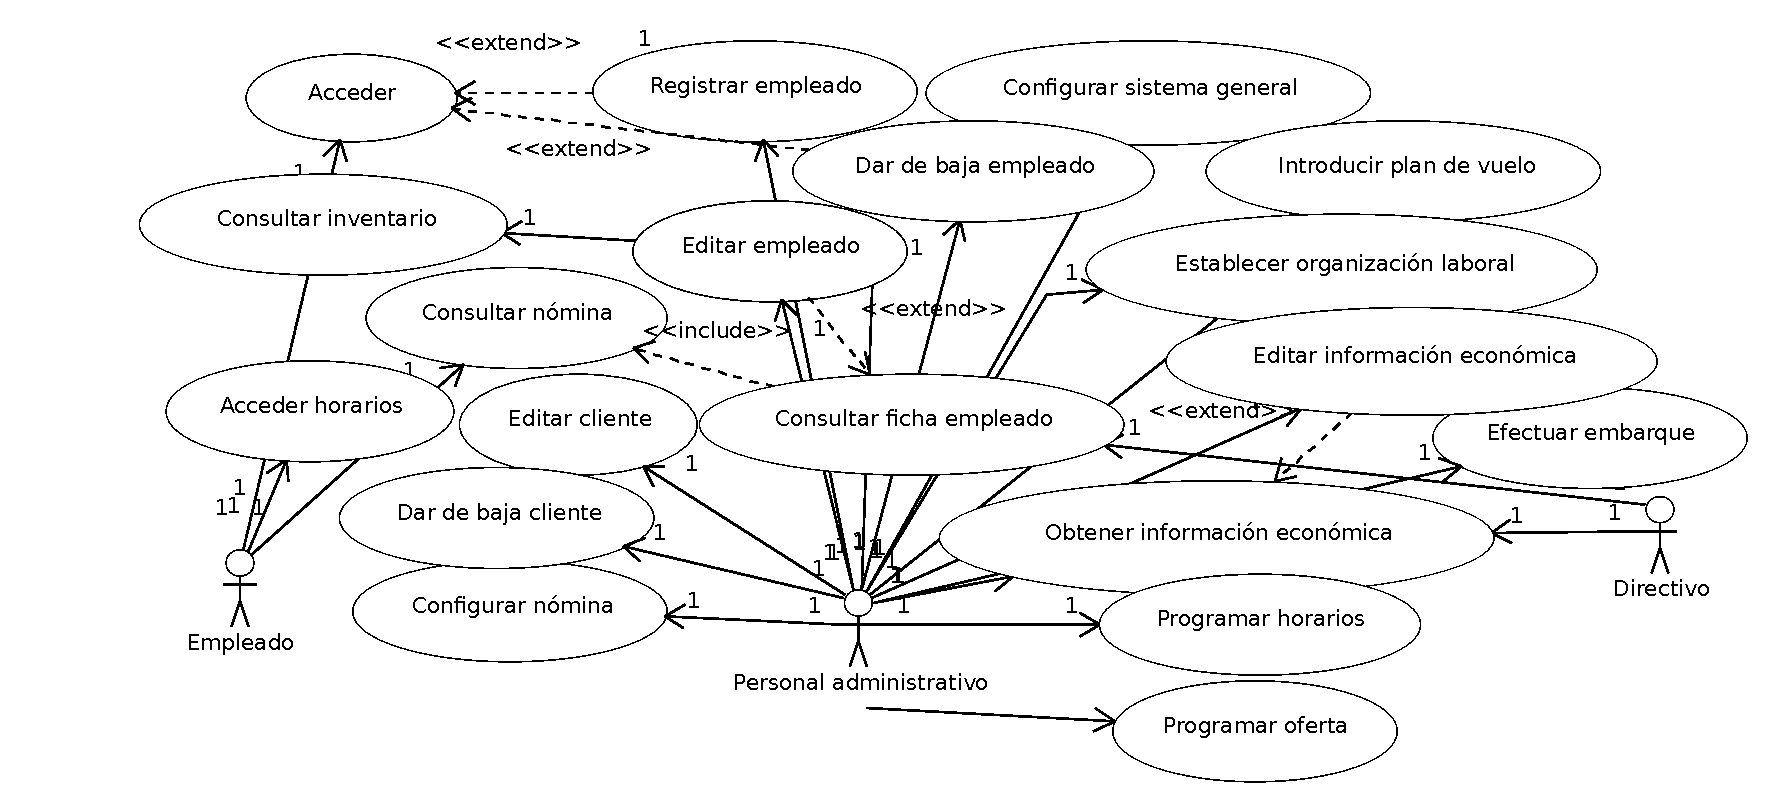
\includegraphics[scale=.45]{gestioninterna1.pdf}
	\end{figure}
\end{frame}

\begin{frame}
	\frametitle{Gestión Interna \scriptsize{Diagrama 2}}

	\begin{figure}
		\hspace*{-.3cm}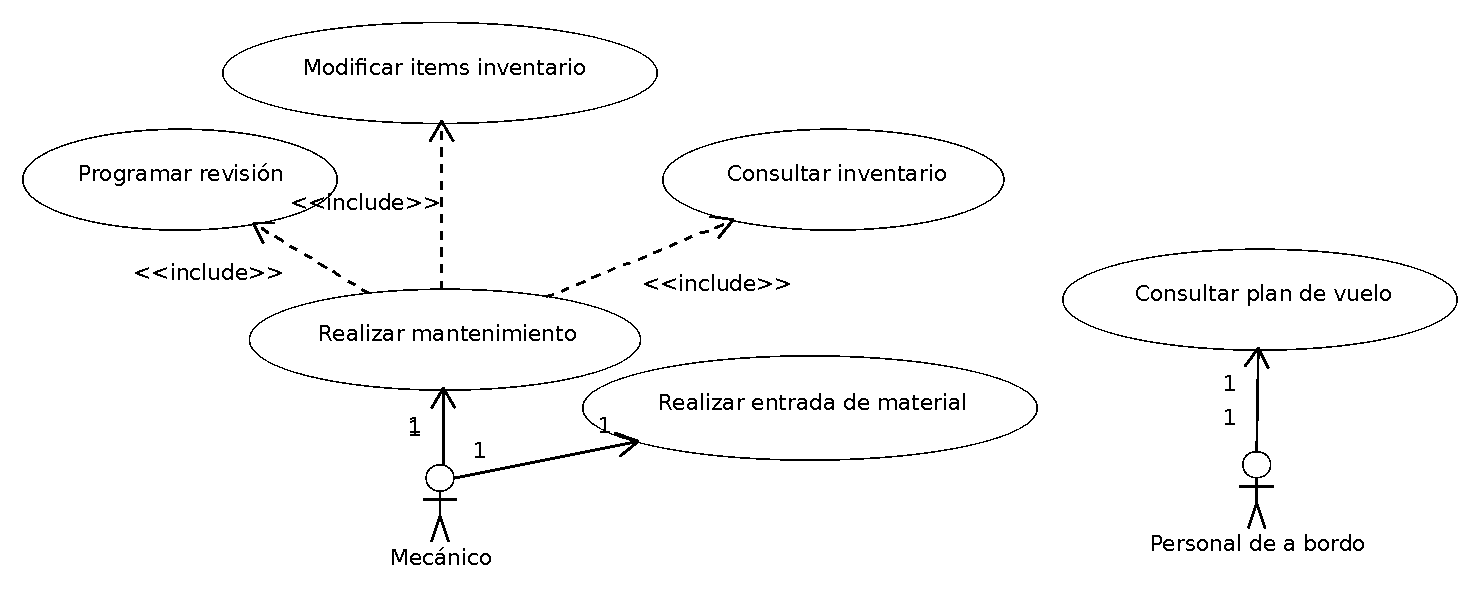
\includegraphics[scale=.5]{gestioninterna2.pdf}
	\end{figure}
\end{frame}

\begin{frame}
	\frametitle{Gestión Externa \scriptsize{Diagrama}}

	\begin{figure}
		\hspace*{-.2cm}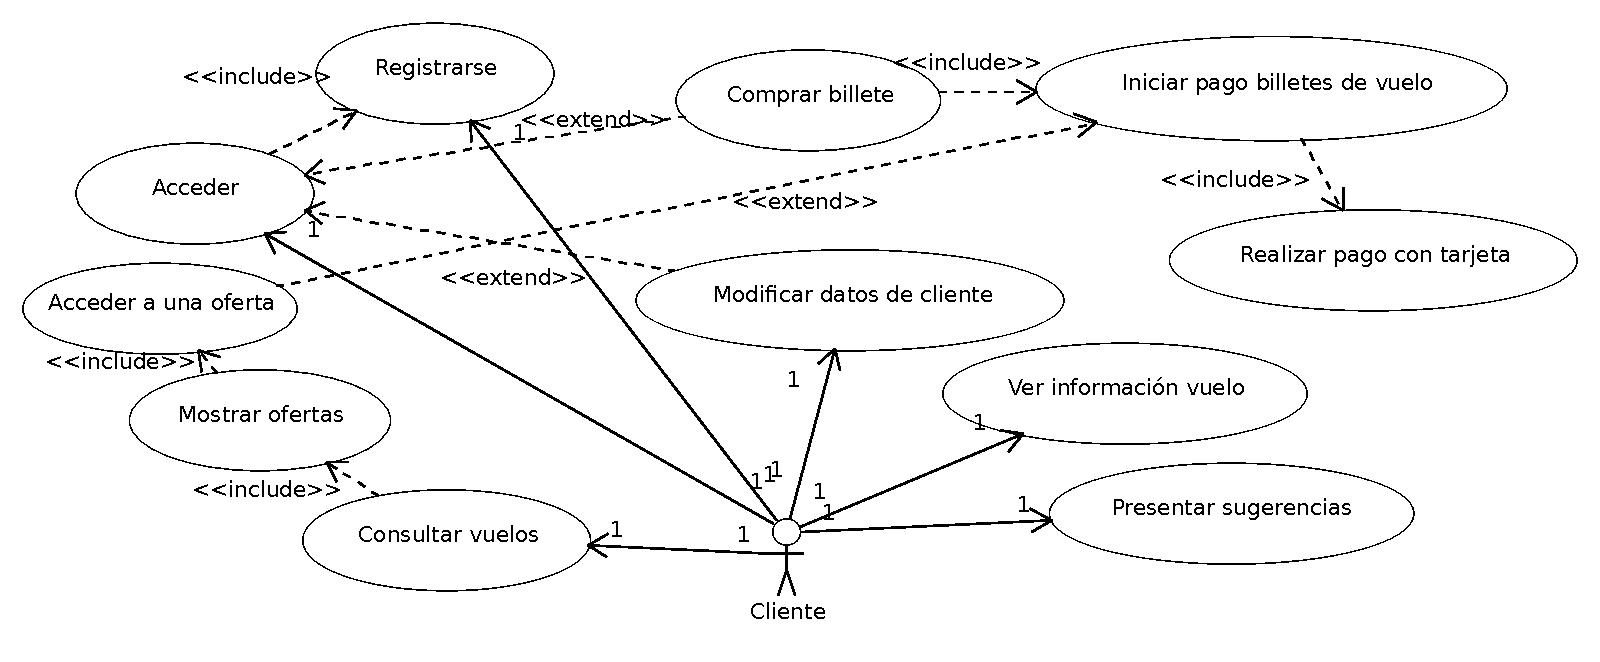
\includegraphics[scale=.46]{gestionexterna.pdf}
	\end{figure}
\end{frame}

\begin{frame}
	\frametitle{Proceso de desarrollo}

	\begin{block}{Documentos generados}
	\begin{itemize}
		\item Casos de uso \pause
		\item Especificación de requisitos \software (SRS) {\scriptsize IEEE Std 830-1998} \pause
		\item Prototipos
			\begin{itemize}
				\item Interfaz interna
				\item Sitio web
			\end{itemize}
	\end{itemize}
	\end{block}
\end{frame}

\begin{frame}
	\frametitle{Integrantes del Grupo Diedral}

	\begin{block}{Integrantes}
		\begin{itemize}
			\item Cristina Alonso Fernández
			\item Natalia Angulo Herrera
			\item Sandra Bermejo Cañadas
			\item Juan Andrés Claramunt Pérez
			\item Rubén Rafael Rubio Cuéllar
		\end{itemize}
	\end{block}
\end{frame}

\end{document}
